\section{Reinforcement Learning Basic Model}
	\begin{figure}[h]
	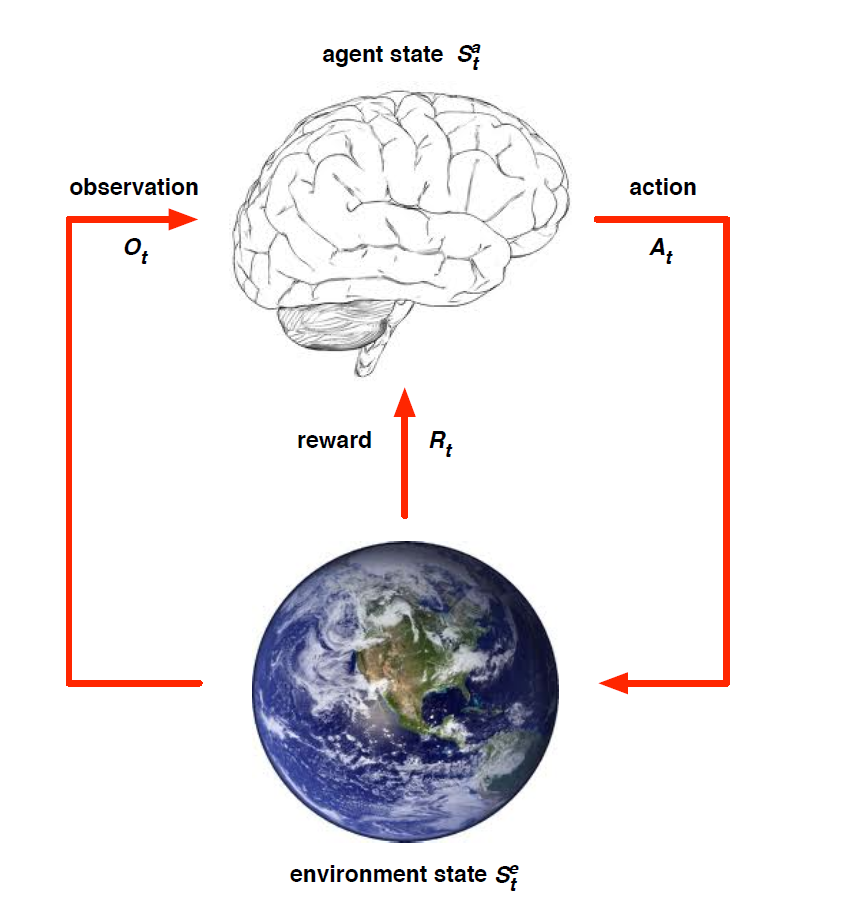
\includegraphics[scale=0.5]{model.png}
	\centering
	\caption{Basic Model of RL}
	\end{figure}
	The \underline{goal} gere is to select a set of \textbf{actions} $ \left\{ A_1, A_2, A_3 ... A_t \right\} $ to maximize total future reward $R_t$ based on the observations $O_t$. Since actions have long-term consequences and reward may be delayed, we cannot approach this problem greedily.

	\paragraph{Definition} \textbf{History} is the sequence of observation, actions and rewards. i.e. 
	\begin{equation*} % * denotes no numbering 
	H_t = A_1, O_1, R_1, A_2, O_2, R_2, ... , A_t, O_t, R_t
	\end{equation*}

	\paragraph{Definition} A \textbf{state} contains the information that \underline{determines} what happens next (i.e. $A_{t+1}, O_{t+1}, R_{t+1}$), and is defined as a function of the history.
	\begin{equation*}
	S_t = f(H_t)
	\end{equation*}

	\paragraph{Definition} The \textbf{environmental state}, $S^e_t$ , is the information that \underline{determines} the next observation $O_{t+1}$ and reward $R_{t+1}$ produce by the environment. Usually not visible to agent.

	\paragraph{Defintition} The \textbf{agent state}, $S^a_t$, is the information that \underline{determines} the next action $A_{t+1}$ produce by the agent, which is often a function of history. i.e. $S^a_t = f(H_t)$

	\subsection{Information State}
	\paragraph{Definition} The \textbf{information state} (a.k.a \textbf{Markov state}) contains all useful information from the history. Given the present, the future is independent of the past. The Markove state is a sufficient statistic of the future.  More formally, the state $S_t$ is \textbf{Markov} i.f.f 
	\begin{equation}
	\mathbb{P} [S_{t+1} | S_t] = \mathbb{P} [S_{t+1} | S_1, S_2, S_3, ..., S_{t-1}, S_t]
	\end{equation}
	The environmental state is Markov (by definition). 
	\paragraph{Proposition} The history is also Markov. 
	\subparagraph{Proof}
	\begin{align*}
	\mathbb{P} [H_{t+1} | H_1, ..., H_t]
	=  &\mathbb{P} [H_{t+1} | A_1, O_1, R_1, A_1, O_1, R_1, A_2, O_2, R_2, ... ,\\
	 	&A_1, O_1, R_1, A_2, O_2, R_2, ..., A_t, O_t, R_t ] \\
	= &\mathbb{P} [H_{t+1} | A_1, O_1, R_1, A_2, O_2, R_2, A_3, O_3, R_3 ..., A_t, O_t, R_t ] \\
	= &\mathbb{P} [H_{t+1} | H_t]
	\end{align*} 

	\subsection{Observability}

 	An environment is \textbf{fully observable} if agent can directly observe the environment state. i.e. $S^a_t = O_t = S^e_t$. Formally known as Markov Decision Process (MDP).\\
 	An environment is \textbf{partially observable} agent indirectly observe the environment. $S^a_t \ne S^e_t $. Formally known as Partially Observable Markov Decision Process (POMDP). We can construct the agent state $S^a_t$ by using:
	\begin{itemize}
	\item Complete History: $S^a_t = H_t$
	\item Beliefs on environment state: $S^a_t = (\mathbb{P}[S^e_t = s_1],...,\mathbb{P}[S^e_t = s_n] )$
	\item Recurrent Neural Network $S^a_t = \sigma(S^a_{t-1} W_s + O_t W_o)$
	\end{itemize}

	\subsection{Components of RL agent}
	\paragraph{Definition} Policy is the mapping of \textbf{state} to \textbf{action}
	\begin{itemize}
	\item Deterministic Policy: $a = \pi(s)$
	\item Probabilisitc Policy $ \pi(\mathbf{a|s}) = \mathbb{P}[A_t|S_t] $
	\end{itemize}
	\paragraph{Definition} A \textbf{Value Function} is a function \textbf{associate with each policy} used to \underline{evalulate} how good the states are, therefore use to select actions. Formally,
	\begin{equation*}
	v_{\pi}(s) = \mathbb{E}[R_{t+1} + \gamma R_{t+2} + \gamma^2R_{t+3} + ... | S_t = s]
	\end{equation*}
	\paragraph{Definition} A model predicts what the \textbf{environment} will do next.
	\begin{itemize}
	\item Transition Probability. The probaility of going from a state to another.
	\begin{equation*}
	\mathcal{P}^a_{ss'} = \mathbb{P}[S_{t+1} = s' | S_t = s, A_t = a]
	\end{equation*}
	\item Emission Probability. The expected reward obtained from the current state. 
	\begin{equation*}
	\mathcal{R}^a_s = \mathbb{E}[R_t | S_t = s, A_t = a]
	\end{equation*}
	 \end{itemize}

	 \subsection{Learning and Planning}
	 If the environment is initially \underline{unknown}, then we need \textbf{learning} by interact with the environment to improve the policy. A.k.a Exploration.\\ 
	 Conversely, if the environment is \underline{known}, all wee need is to perform computations (query) the model to improve the policy. This is known as \textbf{planning} (a.k.a exploitation). 
	 \begin{enumerate}
	 \item Query the emulator.
	 \item If action a is taken from state s, what is the score and what is the next state? 
	 \item Do tree search to find the optimal policy.
	 \end{enumerate}